\documentclass[12pt]{book}

\usepackage[margin=1.1in]{geometry}
\usepackage{amsmath, amssymb, mathtools}
\usepackage{tikz}
\usepackage{enumitem}
\usepackage{xcolor}
\usepackage{mdframed}
\usepackage{epigraph}
\usepackage[colorlinks=true, linkcolor=blue!50!black, citecolor=blue!50!black]{hyperref}

\setlength{\epigraphwidth}{0.85\textwidth}

\definecolor{mottoblue}{RGB}{235,242,250}
\definecolor{mottoline}{RGB}{70,110,160}

\newmdenv[
  backgroundcolor=mottoblue,
  linecolor=mottoline,
  linewidth=1pt,
  roundcorner=4pt,
  innertopmargin=10pt,
  innerbottommargin=10pt,
  innerleftmargin=12pt,
  innerrightmargin=12pt,
  skipabove=14pt,
  skipbelow=14pt
]{mottobox}

\newcounter{reflectq}
\newenvironment{reflectquestions}
  {\begin{list}{\textbf{\arabic{reflectq}.}}
    {\usecounter{reflectq}\setlength{\leftmargin}{1.6em}\setlength{\itemsep}{6pt}}}
  {\end{list}}

\begin{document}

\chapter[Space, Time, and Motion]{Space, Time, and Motion: What We Measure, Not What They Are}
\label{ch:space-time-motion}

\begin{mottobox}
\noindent\textit{``We do not know what space, time, and motion are --- but we know how to measure them.''}

\vspace{4pt}
\noindent\small This sentence is not a single line Feynman wrote down; it is the working motto of physics itself, and Feynman stated its three parts separately, in three different lectures, about three different things. This chapter tells that story and asks what it means for the rest of the subject you are about to study.
\end{mottobox}

\section{A Motto in Three Parts}
\label{sec:motto-origins}

Open almost any introductory physics course and you will be handed, within the first few pages, definitions of space, time, and motion. You will be told that time is ``what a clock measures,'' that length is ``what a ruler measures,'' and that velocity is ``the rate of change of position.'' If you find these definitions strangely circular --- clocks measure time, but what \emph{is} time? --- you are in good company. So did Richard Feynman, and so did every serious physicist since Galileo.

In the opening lectures of \emph{The Feynman Lectures on Physics}, Feynman confronts this circularity head-on, not once but three times, for three different concepts.

On \textbf{energy}, in a lecture on its conservation, he is blunt: it is important to realize that in physics today, he says, ``we have no knowledge of what energy is''\footnote{R. P. Feynman, R. B. Leighton, and M. Sands, \emph{The Feynman Lectures on Physics}, Vol.~I, Ch.~4, \S4.1 (Addison-Wesley, 1963; New Millennium Edition, Caltech, 2013).} --- we only have formulas that let us calculate a number, before and after some process, and find that the number has not changed.

On \textbf{time}, wrestling with the fact that no dictionary definition of time is any good (Webster's circles back on itself), he concludes that what matters is ``not how we define time, but how we measure it''\footnote{Ibid., Ch.~5, \S5.1, ``Time.''} --- and spends the rest of the lecture on clocks, not metaphysics.

On \textbf{motion} and definition generally, after a philosophical detour about whether a moving object is the ``same'' object from moment to moment, he throws up his hands in a way every working scientist will recognize: ``We cannot define anything precisely!''\footnote{Ibid., Ch.~8, \S8.1, ``Description of motion.''} What rescues physics from paralysis, he goes on, is that we do not need a precise definition of a \emph{thing} in order to make precise \emph{measurements} of it.

Put the three together and you get the motto at the top of this chapter. It is not a slogan Feynman coined; it is a description of what he --- and every physicist working in his tradition --- actually \emph{does}. This chapter takes that practice seriously as a method, and applies it to the three concepts that every subsequent chapter of this book will depend on: space, time, and motion.

\section{From Essence to Procedure}
\label{sec:operationalism}

The habit of answering ``how do we measure it?'' instead of ``what is it, really?'' is not obvious, and it is not old. For roughly two thousand years, natural philosophy asked the second kind of question almost exclusively. Aristotle's physics is a physics of essences: a stone falls because it is in its nature to seek the center of the universe; motion needs a mover in constant contact with the moved thing, because motion \emph{is} the actualization of a potential, and potentials need agents. These are answers to ``what is it,'' argued from armchairs, and for two millennia they were taken as settled.

Galileo changed the question. Rather than asking what motion \emph{is}, he rolled a ball down an inclined trough and asked how far it went in how long a time\footnote{Ibid., Ch.~5, \S5.1. Galileo's earliest timing of falling and rolling bodies reportedly used his own pulse, since no accurate short-interval clock yet existed.}. The philosophical question --- is motion the actualization of potential, does a projectile carry an internal \emph{impetus} --- was quietly set aside in favor of a table of numbers: distance against time. It turned out that the numbers were enough. From them Galileo extracted a law ($d \propto t^2$ for constant acceleration) that Aristotelian essences had never produced and, arguably, never could have produced, because essences do not generate numbers.

This is the birth of physics as we now practice it: a science that trades unanswerable questions about the nature of things for answerable questions about relations between measurements. Two and a half centuries later, the American physicist Percy Bridgman gave this practice a name and a philosophy, \emph{operationalism}: the meaning of a physical concept \emph{is} the set of operations used to measure it, nothing more and nothing less\footnote{P. W. Bridgman, \emph{The Logic of Modern Physics} (Macmillan, 1927).}. Bridgman was largely systematizing something Einstein had already done in practice in 1905, and something Galileo had already done in practice in 1604 --- this chapter's motto is simply the physicist's folk memory of that long habit.

It is worth being honest about what this stance is \emph{not}. It is not a claim that space, time, and motion are ``unreal,'' or that physics has given up on understanding the world. It is the much more modest and much more powerful claim that our understanding is built \emph{entirely out of} measurement relations, and that when a concept resists operational definition --- as absolute simultaneity eventually did, in Section~\ref{sec:einstein} --- the fault lies with the concept, not with the measurements.

\section{Measuring Space}
\label{sec:space}

Ask a beginning student what a metre ``is,'' and you are likely to hear a shrug. Ask how to measure one, and you get a procedure. That procedure has changed four times in recorded history, and each change is a small case study in operationalism.

\begin{enumerate}[label=(\roman*)]
  \item \textbf{1793}: the metre is defined as one ten-millionth of the distance from the North Pole to the Equator along the meridian through Paris. Space is measured against the Earth itself.
  \item \textbf{1889}: the metre becomes the distance between two scratches on a specific bar of platinum--iridium alloy, kept in a vault outside Paris. Space is now measured against a chosen artifact, because artifacts are more reproducible than surveying a meridian.
  \item \textbf{1960}: the metre is redefined as \(1{,}650{,}763.73\) wavelengths, in vacuum, of a specific orange-red spectral line of krypton-86. Space is now measured against an atomic process, because atoms of a given isotope are more reproducible than any single artifact, anywhere in the universe.
  \item \textbf{1983}: the metre is defined as the distance light travels, in vacuum, in
  \[
    \frac{1}{299\,792\,458}\ \text{second}.
  \]
  Space is now measured against \emph{time}, via a fixed, exact value of the speed of light, \(c = 299{,}792{,}458\ \text{m/s}\) --- itself no longer a measured quantity but a defined constant.
\end{enumerate}

Notice what has \emph{not} changed across two centuries of redefinition: the operational content of ``distance'' is, and has only ever been, a procedure for comparing an unknown length to a standard. What changed is which standard is most reproducible, most universal, and most stable. There is no deeper fact about ``distance itself'' that these four definitions were converging on and finally reached in 1983. There is only an evolving answer to the question ``how do we measure it,'' each version better than the last by the single criterion that matters: any two laboratories, anywhere, doing the same operation, get the same number.

\section{Measuring Time}
\label{sec:time}

Time has followed an almost identical path, and Feynman's own lecture on the subject is where this chapter's second motto-fragment comes from. Early ``clocks'' were anything periodic: the shadow of a gnomon, the dripping of a water clock, the swing of a pendulum once Galileo and Huygens had shown that a pendulum's period is (nearly) independent of its amplitude. Each of these ties the abstract idea of duration to a concrete, repeatable operation: count the periods.

The modern second is the same idea, made almost unimaginably precise. Since 1967 it has been defined as the duration of \(9{,}192{,}631{,}770\) periods of the radiation corresponding to a particular hyperfine transition in a caesium-133 atom. A caesium clock does not \emph{know} what time is any better than a sundial did; it simply provides a periodic operation so reproducible that two caesium clocks, built independently on opposite sides of the planet, tick in agreement to better than one part in \(10^{14}\).

\begin{mdframed}[backgroundcolor=gray!8, linecolor=gray!40, linewidth=0.6pt, roundcorner=3pt]
\textbf{A caution worth stating early.} An operational definition of time answers ``how do two nearby clocks agree?'' It does \emph{not} automatically answer ``how do two \emph{distant} clocks agree?'' --- that second question turns out to require its own operational procedure, and taking that procedure seriously is what leads, in Section~\ref{sec:einstein}, to relativity.
\end{mdframed}

\section{Measuring Motion}
\label{sec:motion}

Once space and time each have an operational meaning, motion inherits one automatically: motion is nothing more than a record of position measurements paired with time measurements. If a particle is at position $x_1$ at time $t_1$, and at position $x_2$ at a later time $t_2$, its average velocity over that interval is defined --- not discovered, \emph{defined} --- as
\[
  \bar v \;=\; \frac{x_2 - x_1}{t_2 - t_1} \;=\; \frac{\Delta x}{\Delta t}.
\]
There is no further fact about ``what velocity really is'' lurking behind this ratio. The ratio \emph{is} the concept, all the way down.

But this simple-looking definition hides an assumption that turns out to be the single most important idea in this chapter: position relative to \emph{what}? A passenger asleep on a train is at rest relative to the train and moving at \(300\ \text{km/h}\) relative to the ground. Neither statement is more ``true'' than the other; each is the correct output of a well-specified measurement procedure, with the reference frame stated as part of the procedure. This was Galileo's other great insight (again from rolling balls, this time in a ship's cabin): the laws of mechanics look the same in every frame moving at constant velocity, so no experiment performed inside a closed cabin can tell you whether the ship is docked or sailing smoothly. There is no experiment --- no measurement procedure --- that picks out one frame as the ``real'' one. Consequently, physics does not grant the concept of absolute rest any operational meaning, and a mature theory of motion simply drops it.

Figure~\ref{fig:worldline} shows the same idea in the language you will use for the rest of this book: a \emph{spacetime diagram}, with position plotted horizontally and time plotted vertically. A particle at rest traces a vertical line; a particle in uniform motion traces a tilted line, called its \emph{worldline}, whose slope encodes the velocity you just defined above.

\begin{figure}[h]
\centering
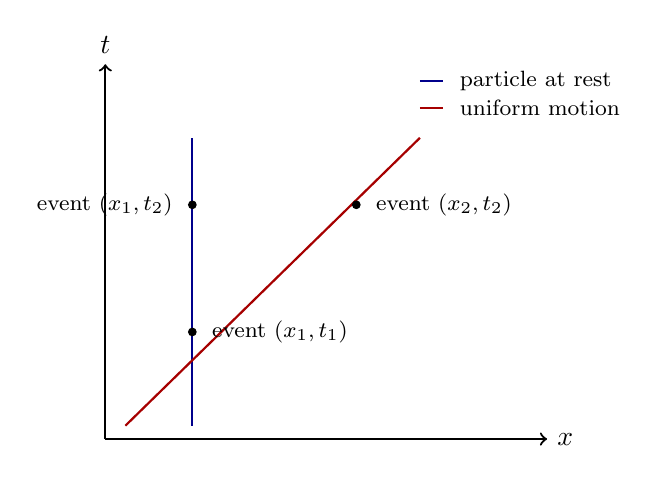
\begin{tikzpicture}[scale=0.85, every node/.style={font=\footnotesize}]
  % axes
  \draw[->, thick] (0,0) -- (6.6,0) node[right, font=\normalsize] {$x$};
  \draw[->, thick] (0,0) -- (0,5.6) node[above, font=\normalsize] {$t$};

  % stationary worldline (x = 1.3, constant)
  \draw[thick, blue!55!black] (1.3,0.2) -- (1.3,4.5);

  % moving worldline (uniform velocity)
  \draw[thick, red!65!black] (0.3,0.2) -- (4.7,4.5);

  % event markers: rest particle at t1 and t2; moving particle at t2
  \filldraw[black] (1.3,1.6) circle (1.6pt);
  \node[anchor=west] at (1.45,1.6) {event $(x_1,t_1)$};

  \filldraw[black] (1.3,3.5) circle (1.6pt);
  \node[anchor=east] at (1.15,3.5) {event $(x_1,t_2)$};

  \filldraw[black] (3.75,3.5) circle (1.6pt);
  \node[anchor=west] at (3.9,3.5) {event $(x_2,t_2)$};

  % compact legend, top right, clear of both lines and the axes
  \draw[thick, blue!55!black] (4.7,5.35) -- (5.05,5.35);
  \node[anchor=west] at (5.15,5.35) {particle at rest};
  \draw[thick, red!65!black] (4.7,4.95) -- (5.05,4.95);
  \node[anchor=west] at (5.15,4.95) {uniform motion};
\end{tikzpicture}
\caption{A spacetime diagram: position on the horizontal axis, time on the vertical axis. Each point is an \emph{event} --- something that happens at a particular place and a particular time. A particle's history is the line, or \emph{worldline}, connecting the events it passes through. The slope of a worldline is the inverse of a velocity: steep and vertical means at rest; increasingly tilted means increasingly fast.}
\label{fig:worldline}
\end{figure}

Two observers moving relative to one another will, in general, assign different velocities to the same particle. Nineteenth-century physics resolved this with a simple addition rule (the \emph{Galilean transformation}): if frame $S'$ moves at speed $v$ relative to frame $S$, then
\[
  x' = x - vt, \qquad t' = t.
\]
Positions transform; time, notice, does not --- it was assumed to be the one measurement every observer would agree on regardless of motion. That second assumption looks so obviously correct that it went unexamined for two hundred years. Section~\ref{sec:einstein} is about what happened when someone finally examined it.

\section[When the Procedure Redefines the Object]{When the Procedure Redefines the Object: Einstein's Radical Consistency}
\label{sec:einstein}

By the standards of Section~\ref{sec:operationalism}, ``two distant events happen at the same time'' is a claim, and claims need an operational meaning: a procedure by which two observers could actually check it. In 1905, Einstein supplied one, and it is disarmingly simple. Place identical clocks at the two locations. Synchronize them by sending a light signal from a point exactly halfway between them, and setting both clocks to read the same time the instant the signal arrives at each. Two events are then defined to be simultaneous, for that observer, if their so-synchronized clocks read the same time when each event occurs.

This is exactly the kind of move this whole chapter has been building toward: instead of asking what simultaneity \emph{is}, ask how you would check it. And the moment you do, something surprising falls out. An observer moving relative to the first one, performing the identical light-signal procedure with clocks at rest \emph{in her own frame}, will synchronize her clocks differently --- because the light signal that looks like it travels equal distances in equal times to the first observer does \emph{not} look that way to the second, who is moving relative to the point of emission. Two events the first observer calls simultaneous, the second observer, using an equally valid procedure, does not.

Simultaneity, length, and duration turn out not to be properties of events themselves, but relations between events and the frame doing the measuring. Take the Galilean transformation of the previous section, insist that every observer must measure the \emph{same} speed of light $c$ by the \emph{same} kind of procedure (this is now an experimentally forced requirement, not a philosophical preference), and the transformation that survives is not the old one but the Lorentz transformation:
\[
  x' = \gamma\,(x - vt), \qquad t' = \gamma\left(t - \frac{vx}{c^2}\right), \qquad \gamma = \frac{1}{\sqrt{1 - v^2/c^2}}.
\]
You will derive and use this transformation properly in a later chapter. For now, notice only its shape: time, which the Galilean transformation left alone, now mixes with space in exactly the symmetric way that space mixed with itself under rotations. Feynman's ``blobs'' of Chapter~17 of his own lectures put it memorably: an object's extension in space and its extension in time turn out to be two faces of one thing, called \emph{spacetime}, in the same way that an object's width and depth are two faces of one thing once you allow yourself to walk around it.

None of this is exotic or merely theoretical. The satellites that make GPS navigation work carry atomic clocks that run measurably faster than identical clocks on the ground, for two combined relativistic reasons (their orbital speed, and their weaker gravity) --- and the correction, on the order of $38\ \mu\text{s}$ per day, is programmed directly into the system, because leaving it out would make GPS positions drift by kilometres within a single day. A phone in your pocket checks Einstein's operational redefinition of time dozens of times a second.

\section{The Deeper Lesson}
\label{sec:lesson}

Return, finally, to energy, where this chapter began. Feynman's point about energy was not a special defeat, confined to one especially slippery concept. It was a preview of the method this whole chapter has described. Physics does not possess, and does not need, an answer to ``what is energy,'' ``what is space,'' ``what is time,'' or ``what is motion,'' in the sense a philosopher might want. What it possesses instead is a set of procedures --- rulers and light signals for space, caesium transitions for time, position-versus-time records for motion, conserved numerical totals for energy --- that are precise, that are shareable between any two observers anywhere, and that let you predict, correctly, what a measurement will read before you have made it.

This is not a modest consolation prize. It is the entire reason physics works. A definition of ``space'' in terms of essence cannot be checked by two different laboratories and cannot be improved when a better standard becomes available; a definition of ``space'' in terms of a measurement procedure can be checked, can be improved, and --- as Section~\ref{sec:einstein} shows --- can even be pushed hard enough to reveal that two of your oldest and most trusted concepts, space and time, were never fully separate to begin with. Every quantitative law you will meet in the rest of this book --- Newton's laws, Maxwell's equations, the Schr\"odinger equation --- is built the same way: not as a statement about the hidden essence of matter, motion, or field, but as a precise relation between things that can be measured. Learning to ask ``how would I measure that?'' before asking ``what is that, really?'' is, more than any single formula, the actual content of learning physics.

\bigskip
\noindent\textbf{Reflection Questions}
\begin{reflectquestions}
\item The 1793 and 1983 definitions of the metre both aim to fix ``the same'' length, yet they specify completely different procedures. In what sense, if any, is it meaningful to ask which one is the ``true'' metre?
\item Bridgman's operationalism says a concept's meaning \emph{is} its measurement procedure. Can you think of a physical concept used casually in everyday language --- for example, ``force,'' ``hot,'' or ``heavy'' --- that does \emph{not} yet have a single agreed operational definition? What problems does that ambiguity cause?
\item Section~\ref{sec:motion} argues that no measurement can detect absolute rest. Explain, in your own words, why a passenger on a smoothly sailing ship cannot perform \emph{any} experiment, purely mechanical, that reveals whether the ship is moving.
\item Explain why Einstein's light-signal synchronization procedure, applied by two observers in relative motion, must give different answers about which pairs of distant events are simultaneous. (Hint: focus on what stays the same for both observers, and what does not.)
\item Feynman says physics has ``no knowledge of what energy is,'' yet energy is one of the most successful concepts in all of science. Reconcile these two statements in two or three sentences.
\end{reflectquestions}

\bigskip
\begin{thebibliography}{9}

\bibitem{feynman}
R.~P.~Feynman, R.~B.~Leighton, and M.~Sands,
\emph{The Feynman Lectures on Physics}, Vol.~I, New Millennium Edition (Caltech, 2013), Chs.~4, 5, 8, 17.
\url{https://www.feynmanlectures.caltech.edu/}

\bibitem{bridgman}
P.~W.~Bridgman, \emph{The Logic of Modern Physics} (Macmillan, 1927).

\bibitem{einstein1905}
A.~Einstein, ``Zur Elektrodynamik bewegter K\"orper,'' \emph{Annalen der Physik} \textbf{17}, 891--921 (1905).

\bibitem{bipm}
Bureau International des Poids et Mesures, \emph{The International System of Units (SI Brochure)}, 9th edition (2019) --- definitions of the metre and the second.

\end{thebibliography}

\end{document}
